\chapter{Procesos de Ingeniería de Software según SWEBOK}

\section{Gestión de la configuración del Software (SCM)}
Imagina que un equipo de chefs está trabajando en la receta de un platillo complejo. 
Al principio, todos tienen una copia de la receta original. 
Pero pronto, un chef decide que necesita un poco más de sal y lo anota en su copia. 
Otro piensa que es mejor hornearlo a una temperatura más alta. 
Un tercero cambia un ingrediente por completo. 
Si no hay un control central, al final del día, nadie sabe cuál es la versión correcta de la receta. 
El resultado es el caos.

La Gestión de la Configuración del Software (SCM) es el sistema que evita este caos. 
Es la disciplina que actúa como la fuente única y fiable de la verdad para todo el proyecto. 
El SWEBOK la define como un proceso de apoyo fundamental que controla la evolución y la integridad del producto a lo largo de su ciclo de vida.

No se trata solo del código fuente. 
La SCM gestiona todos los elementos importantes (llamados ``elementos de configuración'') que definen el software.

\subsection*{Actividades clave de la SCM}
\begin{description}
  \item[Identificación:] ¿Qué vamos a controlar? Es el primer paso, donde se decide qué artefactos son lo suficientemente importantes como para ser gestionados. Esto incluye:
  \begin{itemize}
    \item Código fuente
    \item Documentos de requisitos y de diseño
    \item Casos de prueba y scripts
    \item Manuales de usuario
    \item Incluso las herramientas y compiladores utilizados
  \end{itemize}

  \item[Control de cambios:] ¿Cómo gestionamos las modificaciones? Una vez que un elemento está bajo control, nadie puede cambiarlo sin más. Se establece un proceso formal, a menudo a través de un Comité de Control de Cambios (CCB), para proponer, evaluar y aprobar cualquier modificación. Esto asegura que cada cambio sea deliberado y que su impacto sea bien entendido.

  \item[Contabilidad del estado:] ¿Cuál es el estado actual de todo? Es el proceso de registrar y reportar el estado de cada elemento y de cada solicitud de cambio. Permite a cualquiera saber qué versión es la más reciente, qué cambios se han implementado y cuáles están pendientes. Es el historial completo del proyecto.

  \item[Auditoría de la configuración:] ¿Lo que tenemos es lo que creemos que tenemos? Se realizan auditorías periódicas para verificar que el producto construido coincide con los planos y que se han seguido los procesos establecidos. Es una revisión para asegurar la integridad y la consistencia del producto final.
\end{description}

\section{Planificación y seguimiento de proyectos}
Si la SCM es el mapa detallado del ``qué'' estamos construyendo en un momento dado, 
la planificación y el seguimiento son la brújula y el GPS que nos guían en el ``cómo'' y el ``cuándo'' lo construiremos. 
Es la disciplina de gestión que traza la ruta hacia el objetivo final y se asegura de que no nos desviemos del camino.

El SWEBOK aborda esto como un ciclo continuo. 
Primero planificamos el viaje y luego, durante el trayecto, verificamos constantemente nuestra posición en el mapa.

\subsection*{La planificación}
Esta fase inicial consiste en responder a las preguntas fundamentales que definirán el esfuerzo a realizar. 
No se trata de tener una bola de cristal, sino de utilizar la información disponible para crear una hoja de ruta realista.

\begin{longtable}{p{4cm} p{10cm}}
\caption{Actividades clave de planificación de proyectos} \\
\toprule
\textbf{Actividad clave} & \textbf{Pregunta que responde} \\
\midrule
\endfirsthead

\toprule
\textbf{Actividad clave} & \textbf{Pregunta que responde} \\
\midrule
\endhead

\bottomrule
\endfoot

Definir entregables & ¿Qué vamos a producir exactamente? ¿Cuáles son los productos de trabajo (código, documentos, manuales) que entregaremos al final? \\

Estimación de esfuerzo, calendario y costos & ¿Cuánto trabajo se necesita? ¿Cuánto tiempo nos llevará? ¿Cuál será el presupuesto? \\

Asignación de recursos & ¿Quién hará el trabajo? ¿Qué herramientas y tecnologías necesitamos para llevarlo a cabo? \\

Gestión de riesgos & ¿Qué podría salir mal? ¿Cuáles son los mayores peligros (técnicos, de personal, de mercado) y qué plan tenemos para mitigarlos? \\

Planificación de la calidad & ¿Qué tan bueno debe ser el producto final? ¿Qué procesos de revisión y pruebas implementaremos para alcanzar ese nivel de calidad? \\
\end{longtable}

\subsection*{El seguimiento}
Una vez que el proyecto está en marcha, la planificación no termina. 
El seguimiento es el proceso continuo de:
\begin{itemize}
  \item \textbf{Medir:} Recopilar datos reales sobre el progreso del proyecto. ¿Cuánto hemos gastado? ¿En qué fecha estamos? ¿Qué tareas se han completado?
  \item \textbf{Comparar:} Contrastar los datos reales con lo que se había planificado. ¿Vamos adelantados o retrasados? ¿Estamos por encima o por debajo del presupuesto?
  \item \textbf{Actuar:} Si hay desviaciones significativas, tomar decisiones para corregir el rumbo. Esto puede implicar reasignar recursos, ajustar el calendario o incluso renegociar el alcance del proyecto con el cliente.
\end{itemize}

\section{Modelos de ciclo de vida y procesos}
No hay una única forma de construir software, al igual que no hay una única forma de cocinar. 
La elección del método depende de lo que estés preparando. 
El SWEBOK explica que un modelo de ciclo de vida es, en esencia, la receta maestra que un equipo sigue desde la idea inicial hasta la entrega final del producto. 
Define las fases, las tareas y el orden en que se deben realizar las cosas.

Piensa en ello como la diferencia entre seguir una receta de repostería francesa y cocinar un salteado creativo.

\begin{longtable}{p{3cm} p{6cm} p{6cm}}
\caption{Comparación entre enfoques de ciclo de vida del software} \\
\toprule
\textbf{Característica} & \textbf{Enfoque predictivo} & \textbf{Enfoque adaptativo} \\
\midrule
\endfirsthead

\toprule
\textbf{Característica} & \textbf{Enfoque predictivo} & \textbf{Enfoque adaptativo} \\
\midrule
\endhead

\bottomrule
\endfoot

Planificación & Se realiza de forma exhaustiva al inicio. Se intenta predecir todo el proyecto & La planificación es continua y se ajusta en cada ciclo. Se adapta al cambio \\

Requisitos & Se definen y se ``congelan'' al principio. Son la base inamovible del proyecto & Se aceptan y se dan la bienvenida. Los requisitos evolucionan a medida que se aprende más \\

Entrega & Se realiza una única gran entrega al final del proyecto & Se realizan entregas pequeñas, frecuentes y funcionales (incrementos) de software \\

Gestión del cambio & El cambio se ve como un riesgo que debe ser controlado y minimizado & El cambio se ve como una realidad inevitable y una oportunidad para aportar más valor \\

Rol del cliente & Participa intensamente al principio (requisitos) y al final (aceptación) & Colabora de forma continua con el equipo de desarrollo a lo largo de todo el proyecto \\
\end{longtable}

\section{Aseguramiento de la calidad (SQA)}
Es fácil confundir el Aseguramiento de la Calidad (SQA) con las pruebas, pero son dos cosas muy diferentes. 
El SWEBOK nos ayuda a entender esta distinción crucial.

Por ejemplo, en una fábrica de automóviles:

\begin{itemize}
  \item \textbf{Las pruebas (testing):} Son el inspector al final de la línea de montaje que revisa cada coche antes de que salga de la fábrica. 
  Su trabajo es encontrar defectos en el producto final, como una puerta que no cierra bien o un motor que hace un ruido extraño. 
  Es una actividad reactiva.
  \item \textbf{El aseguramiento de la calidad (SQA):} Es el supervisor de toda la fábrica. 
  No se centra en el coche terminado, sino en el proceso de fabricación. 
  Su trabajo es asegurarse de que las herramientas estén bien calibradas, que los trabajadores estén bien entrenados, que los materiales cumplan los estándares y que los procedimientos de montaje se sigan de manera consistente. 
  Su objetivo es prevenir que los defectos ocurran en primer lugar. 
  Es una actividad proactiva.
\end{itemize}
\begin{figure}[H]
    \centering
    \caption{Proceso de desarrollo de software}
    \label{fig:proceso_software}
    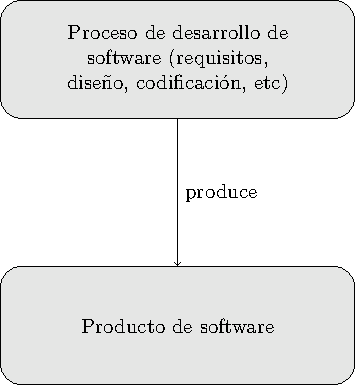
\includegraphics[width=0.4\textwidth]{image/cap2_img1.pdf}
\end{figure}
SQA se enfoca en el proceso. Se pregunta: ``¿Estamos construyendo el producto de la manera correcta?''

Testing se enfoca en el producto. Se pregunta: ``¿Hemos construido el producto correcto?''

\section{Medición y mejora de procesos}
Una famosa frase en el mundo de la gestión dice: 
``Lo que no se mide, no se puede mejorar''. 
Esta idea es el núcleo de este apartado del SWEBOK. 
Sin datos, cualquier intento de mejorar nuestros procesos de desarrollo de software se basa en la intuición, las corazonadas o, en el peor de los casos, en el azar. 
La medición nos proporciona el mapa y la brújula para navegar hacia procesos más eficientes y efectivos.

Imagina que eres el entrenador de un equipo deportivo. 
No te limitarías a decirles a tus jugadores ``¡sean mejores!''. 
Para mejorar de verdad, necesitarías medir su rendimiento:
\begin{itemize}
  \item ¿Cuál es el porcentaje de acierto en los tiros libres?
  \item ¿Cuántos kilómetros corren por partido?
  \item ¿Cuántos pases completan antes de perder el balón?
\end{itemize}

Solo con estos datos puedes identificar debilidades, probar nuevas estrategias (procesos) y medir si esas estrategias están funcionando. 
En la ingeniería de software, el principio es exactamente el mismo.

\subsection*{El Ciclo de la Mejora Continua}
El SWEBOK nos presenta la mejora de procesos no como un evento único, sino como un ciclo continuo y sostenible. 
Uno de los modelos más clásicos para ilustrar esto es el ciclo Planificar-Hacer-Verificar-Actuar (PDCA), también conocido como el ciclo de Deming.
Podemos visualizarlo de la siguiente manera:
\begin{figure}[H]
    \centering
    \caption{Ciclo de la mejora continua}
    \label{fig:ciclo_mejora_continua}
    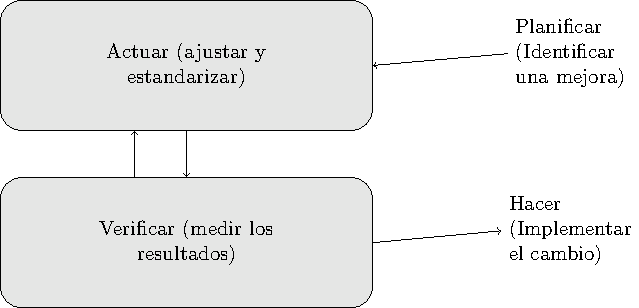
\includegraphics[width=0.6\textwidth]{image/cap2_img2.pdf}
\end{figure}
\begin{description}
  \item[Planificar (Plan):] ¿Qué queremos mejorar? El primer paso es identificar un área de mejora. Esto podría surgir del análisis de datos (por ejemplo, ``estamos encontrando demasiados errores durante las pruebas de sistema'') o de una nueva meta estratégica (``necesitamos reducir el tiempo de entrega en un 15\%''). Se define una hipótesis: ``Si implementamos revisiones de código formales, creemos que el número de errores encontrados en fases tardías disminuirá''.

  \item[Hacer (Do):] Implementar el cambio a pequeña escala. En lugar de cambiar la forma de trabajar de toda la organización de la noche a la mañana, se prueba el nuevo proceso en un entorno controlado. Por ejemplo, se introduce el proceso de revisión de código en un solo equipo o en un solo proyecto piloto.

  \item[Verificar (Check):] ¿Funcionó nuestra hipótesis? Aquí es donde la medición es crucial. Se recopilan datos del proyecto piloto y se comparan con los datos históricos (la línea de base). ¿Se redujo realmente el número de errores encontrados en las pruebas? ¿El esfuerzo extra en las revisiones de código se vio compensado por un menor esfuerzo en la depuración?

  \item[Actuar (Act):] Tomar una decisión basada en los datos. Si el nuevo proceso funcionó, se estandariza y se despliega a otros equipos o a toda la organización. Si no funcionó como se esperaba, se ajusta el proceso y se inicia el ciclo de nuevo con una nueva hipótesis. O quizás, se descarta la idea y se prueba otra diferente.
\end{description}
